
\begin{figure}
\centering

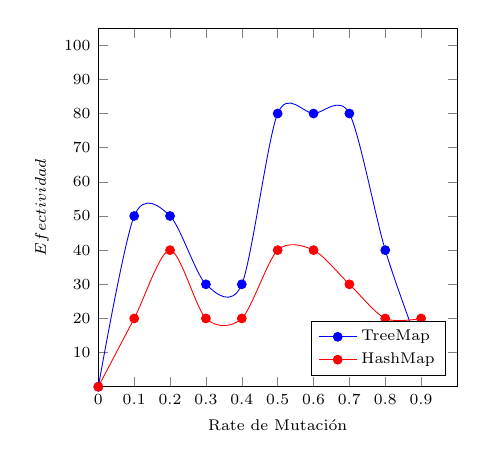
\begin{tikzpicture}[scale=0.8]
\begin{axis}[
    width=0.60\textwidth,
    height=0.60\textwidth,
    xmin=0, xmax=1,
    ymin=0, ymax=105,
    xlabel={\scriptsize{Rate de Mutación}},
    ylabel={\scriptsize{$Efectividad$}},
    xtick={0,0.1,0.2,...,0.9},
    ytick={10,20,...,100},
    legend pos=south east,
    legend cell align={left},
    legend style={font=\scriptsize},
    tick label style={font=\scriptsize}
]

\addplot[mark=*,blue,,smooth] coordinates {
    (0, 0)
    (0.1, 50)
    (0.2, 50)
    (0.3, 30)
    (0.4, 30)
    (0.5, 80)
    (0.6, 80)
    (0.7, 80)
    (0.8, 40)
    (0.9, 10)
};
\addplot[mark=*,red,,smooth] coordinates {
    (0, 0)
    (0.1, 20)
    (0.2, 40)
    (0.3, 20)
    (0.4, 20)
    (0.5, 40)
    (0.6, 40)
    (0.7, 30)
    (0.8, 20)
    (0.9, 20)
};
\legend{TreeMap, HashMap}

\end{axis}
\end{tikzpicture}%
\hfill
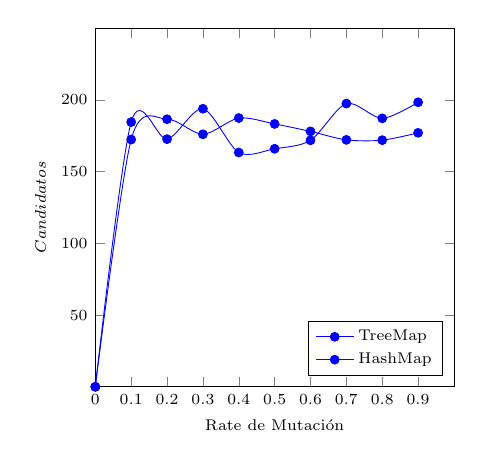
\begin{tikzpicture}[scale=0.8]
\begin{axis}[
    width=0.60\textwidth,
    height=0.60\textwidth,
    xmin=0, xmax=1,
    ymin=0, ymax=250,
    xlabel={\scriptsize{Rate de Mutación}},
    ylabel={\scriptsize{$Candidatos$}},
    xtick={0,0.1,0.2,...,0.9},
    ytick={50,100,150,200},
    legend pos=south east,
    legend cell align={left},
    legend style={font=\scriptsize},
    tick label style={font=\scriptsize}
]

\addplot[mark=*,blue,smooth] coordinates {
    (0,0)
    (0.1, 184.5)
    (0.2, 172.6)
    (0.3, 193.8)
    (0.4, 163.3)
    (0.5, 165.9)
    (0.6, 171.8)
    (0.7, 197.4)
    (0.8, 187.1)
    (0.9, 198.3)
};

\addplot[mark=*,blue,smooth] coordinates {
    (0,0)
    (0.1, 172.3)
    (0.2, 186.5)
    (0.3, 176)
    (0.4, 187.3)
    (0.5, 183.2)
    (0.6, 178)
    (0.7, 172.1)
    (0.8, 171.9)
    (0.9, 177)
};
\legend{TreeMap,HashMap}

\end{axis}
\end{tikzpicture}

\caption{Gráficos de Efectividad y cantidad de candidatos de acuerdo al rate de mutación}
\end{figure}

